When the user edits the spreadsheet, it is the client’s responsibility to push 
those edits to the server so that all of the other clients may be notified 
that the spreadsheet has changed. The client will use the \hyperref[sec:message:push]{push} command to 
update the server with the edits that have been made locally. push accepts 
the id of the spreadsheet to apply the edits to and a list of edits that have 
been made. This command will trigger an update for all clients that currently 
have the spreadsheet open. Each edit will contain the edited contents of one 
or more cells. It is up to the clients how to group the cells into individual 
edits, but the undo command will roll back one full edit, so edits should be 
constructed in such a way that undos will make sense. Edits must be valid 
(cannot cause a circular dependency or formula error) for them to be applied 
to the spreadsheet, so edits must contain enough cells to be valid. For 
example, if including edits from just A1 would cause the edit to be invalid, 
it must also contain new content for cells such that the edit would be valid.

\begin{figure}[H]
    \begin{center}
        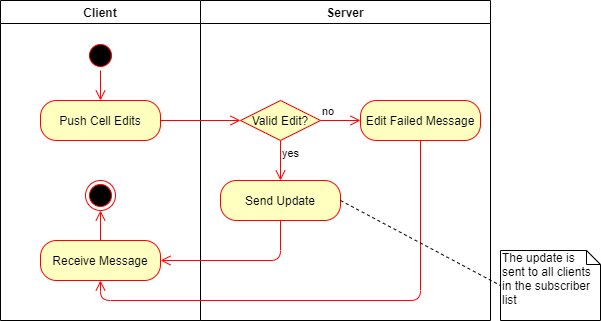
\includegraphics[width=2.5in]{Figures/apply_edit_sprd.png}
        \caption{Update propagation after application of edit}
    \end{center}
\end{figure}